%-------------------------------------------------------------------------------
% 请勿删除本注释
% Free Response Question 1
%
% 指引:
% 如在小问之前有通用问题描述,请放置于此
%-------------------------------------------------------------------------------
\begin{figure}[H]
\centering
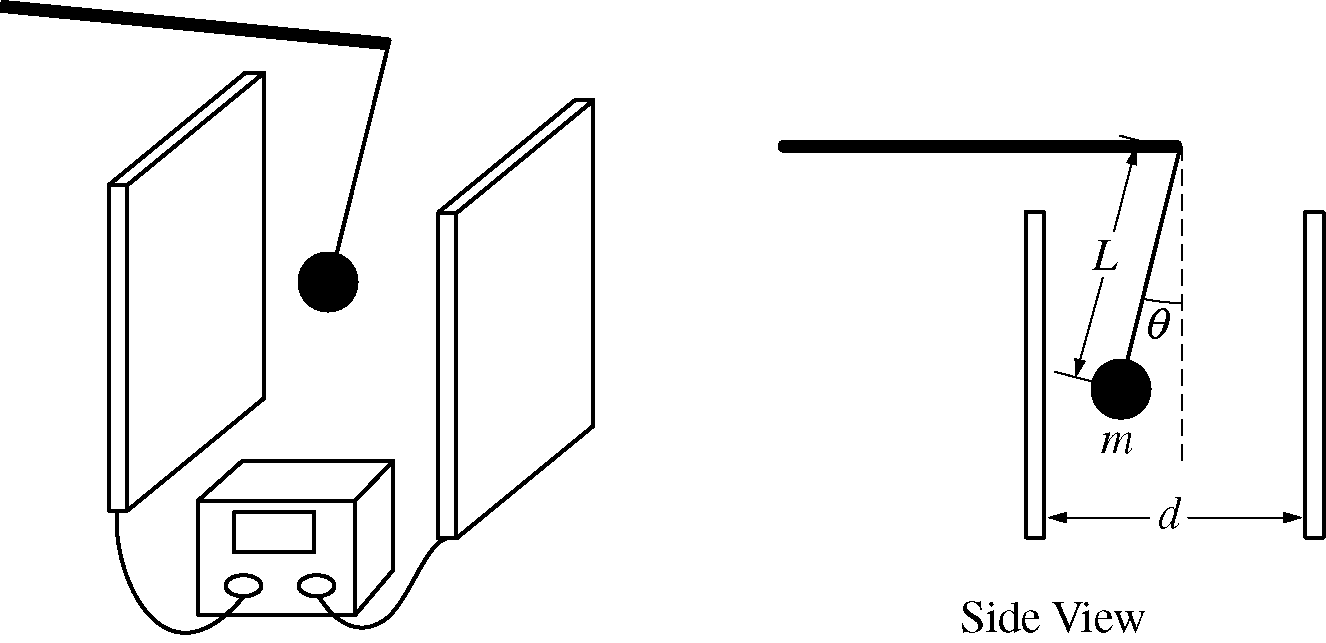
\includegraphics[scale=0.2]{images/img-016-042.png}
\end{figure}


\question
You perform a laboratory experiment to determine the unknown charge on a small conducting ball of mass $m$ using the experimental setup shown in the diagram above. A variable power supply applies a DC voltage to two large parallel plates separated by a distance $d$, creating a uniform electric field. The charged ball hangs between the plates on an insulated thread of length $L$ and is displaced from its lowest point, coming to equilibrium at an angle $\theta$ with the vertical. During the experiment, you measure the angle $\theta$ when the voltage indicated on the power supply is $V$. % 请删除并替换本行,与上一行 \question 之间不要留空行

\begin{parts}

%-------------------------------------------------------------------------------
% 请勿删除本注释
% Part (a)
%
% 指引:
% 如在小问之前有通用问题描述,请放置于此
%-------------------------------------------------------------------------------

\part
On the dot below that represents the conducting ball, draw and label the forces (not components) that act on the conducting ball. Each force must be represented by a distinct arrow starting on, and pointing away from, the dot. % 请删除并替换本行,与上一行 \part 之间不要留空行

\begin{figure}[H]
\centering
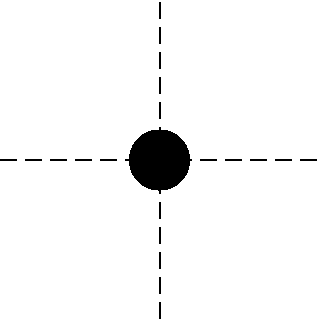
\includegraphics[scale=0.3]{images/img-016-043.png}
\end{figure}


%-------------------------------------------------------------------------------
% 请勿删除本注释
% Part (b)
%
% 指引:
% 如在小问之前有通用问题描述,请放置于此
%-------------------------------------------------------------------------------

\part
Derive an expression that would allow you to calculate the magnitude of the unknown charge on the ball given $\theta, V, m, d, L$, and fundamental constants, as appropriate. If you need to draw anything other than what you have shown in part (a) to assist in your solution, use the space below. Do NOT add anything to the figure in part (a). % 请删除并替换本行,与上一行 \part 之间不要留空行

%-------------------------------------------------------------------------------
% 请勿删除本注释
% Part (c)
%
% 指引:
% 如在小问之前有通用问题描述,请放置于此
%-------------------------------------------------------------------------------

\part
One way to determine a more accurate value for the magnitude of the charge on the conducting ball in the experiment is to perform multiple trials. % 请删除并替换本行,与上一行 \part 之间不要留空行
\begin{subparts}
\subpart What quantity would you vary in this experiment to obtain different values of the angle $\theta$ ?
\subpart What quantities would you plot on a graph to obtain a linear relationship that can be used to determine the magnitude of the charge on the conducting ball?
\end{subparts}

%-------------------------------------------------------------------------------
% 请勿删除本注释
% Part (d)
%
% 指引:
% 如在小问之前有通用问题描述,请放置于此
%-------------------------------------------------------------------------------

\part
Describe one difficulty in precisely and accurately determining the angle $\theta$ with a protractor, and describe a method to overcome the difficulty. % 请删除并替换本行,与上一行 \part 之间不要留空行

%-------------------------------------------------------------------------------
% 请勿删除本注释
% Part (e)
%
% 指引:
% 如在小问之前有通用问题描述,请放置于此
%-------------------------------------------------------------------------------

\part
If the voltage is high enough, the ball touches one of the plates. Describe what happens from the time it touches until you turn off the voltage. % 请删除并替换本行,与上一行 \part 之间不要留空行

\end{parts}


